\section{GPUE: GPU Gross--Pitaevskii equation solver}

Given the effectiveness of GPU computing in completing the simulation of a linear Sch\"odinger equation system, I next applied the newly-developed techniques to simulating Bose--Einstein condensates, which formed the bulk of work during my thesis. The body of work developed for this new project has been realeased as the software tool ``GPUE'', available at \url{https://github.com/mlxd/gpue}. Performance metrics of this code was carried out by Peter Wittek, ICFO, Barcelona [cite website]. The comparison was performed with GPUE, the Trotter-Suzuki package developed by Wittek \textit{et al}, and the mature GPELab software suite for MATLAB [url]. The sample results taken for time evolution are given by Fig.~\ref{fig:gpuevsts}. GPUE and GPU-enabled TS clearly beat MATLAB, and CPU performance by a significant margin. Although TS is a more generalised suite for computing, the GPU computation does not yet allow for states with angular momentum, and so GPUE is currently the optimal choice for two dimensional rotating condensate systems out of the examined software suites.

\begin{figure}[htb]
    \centering
    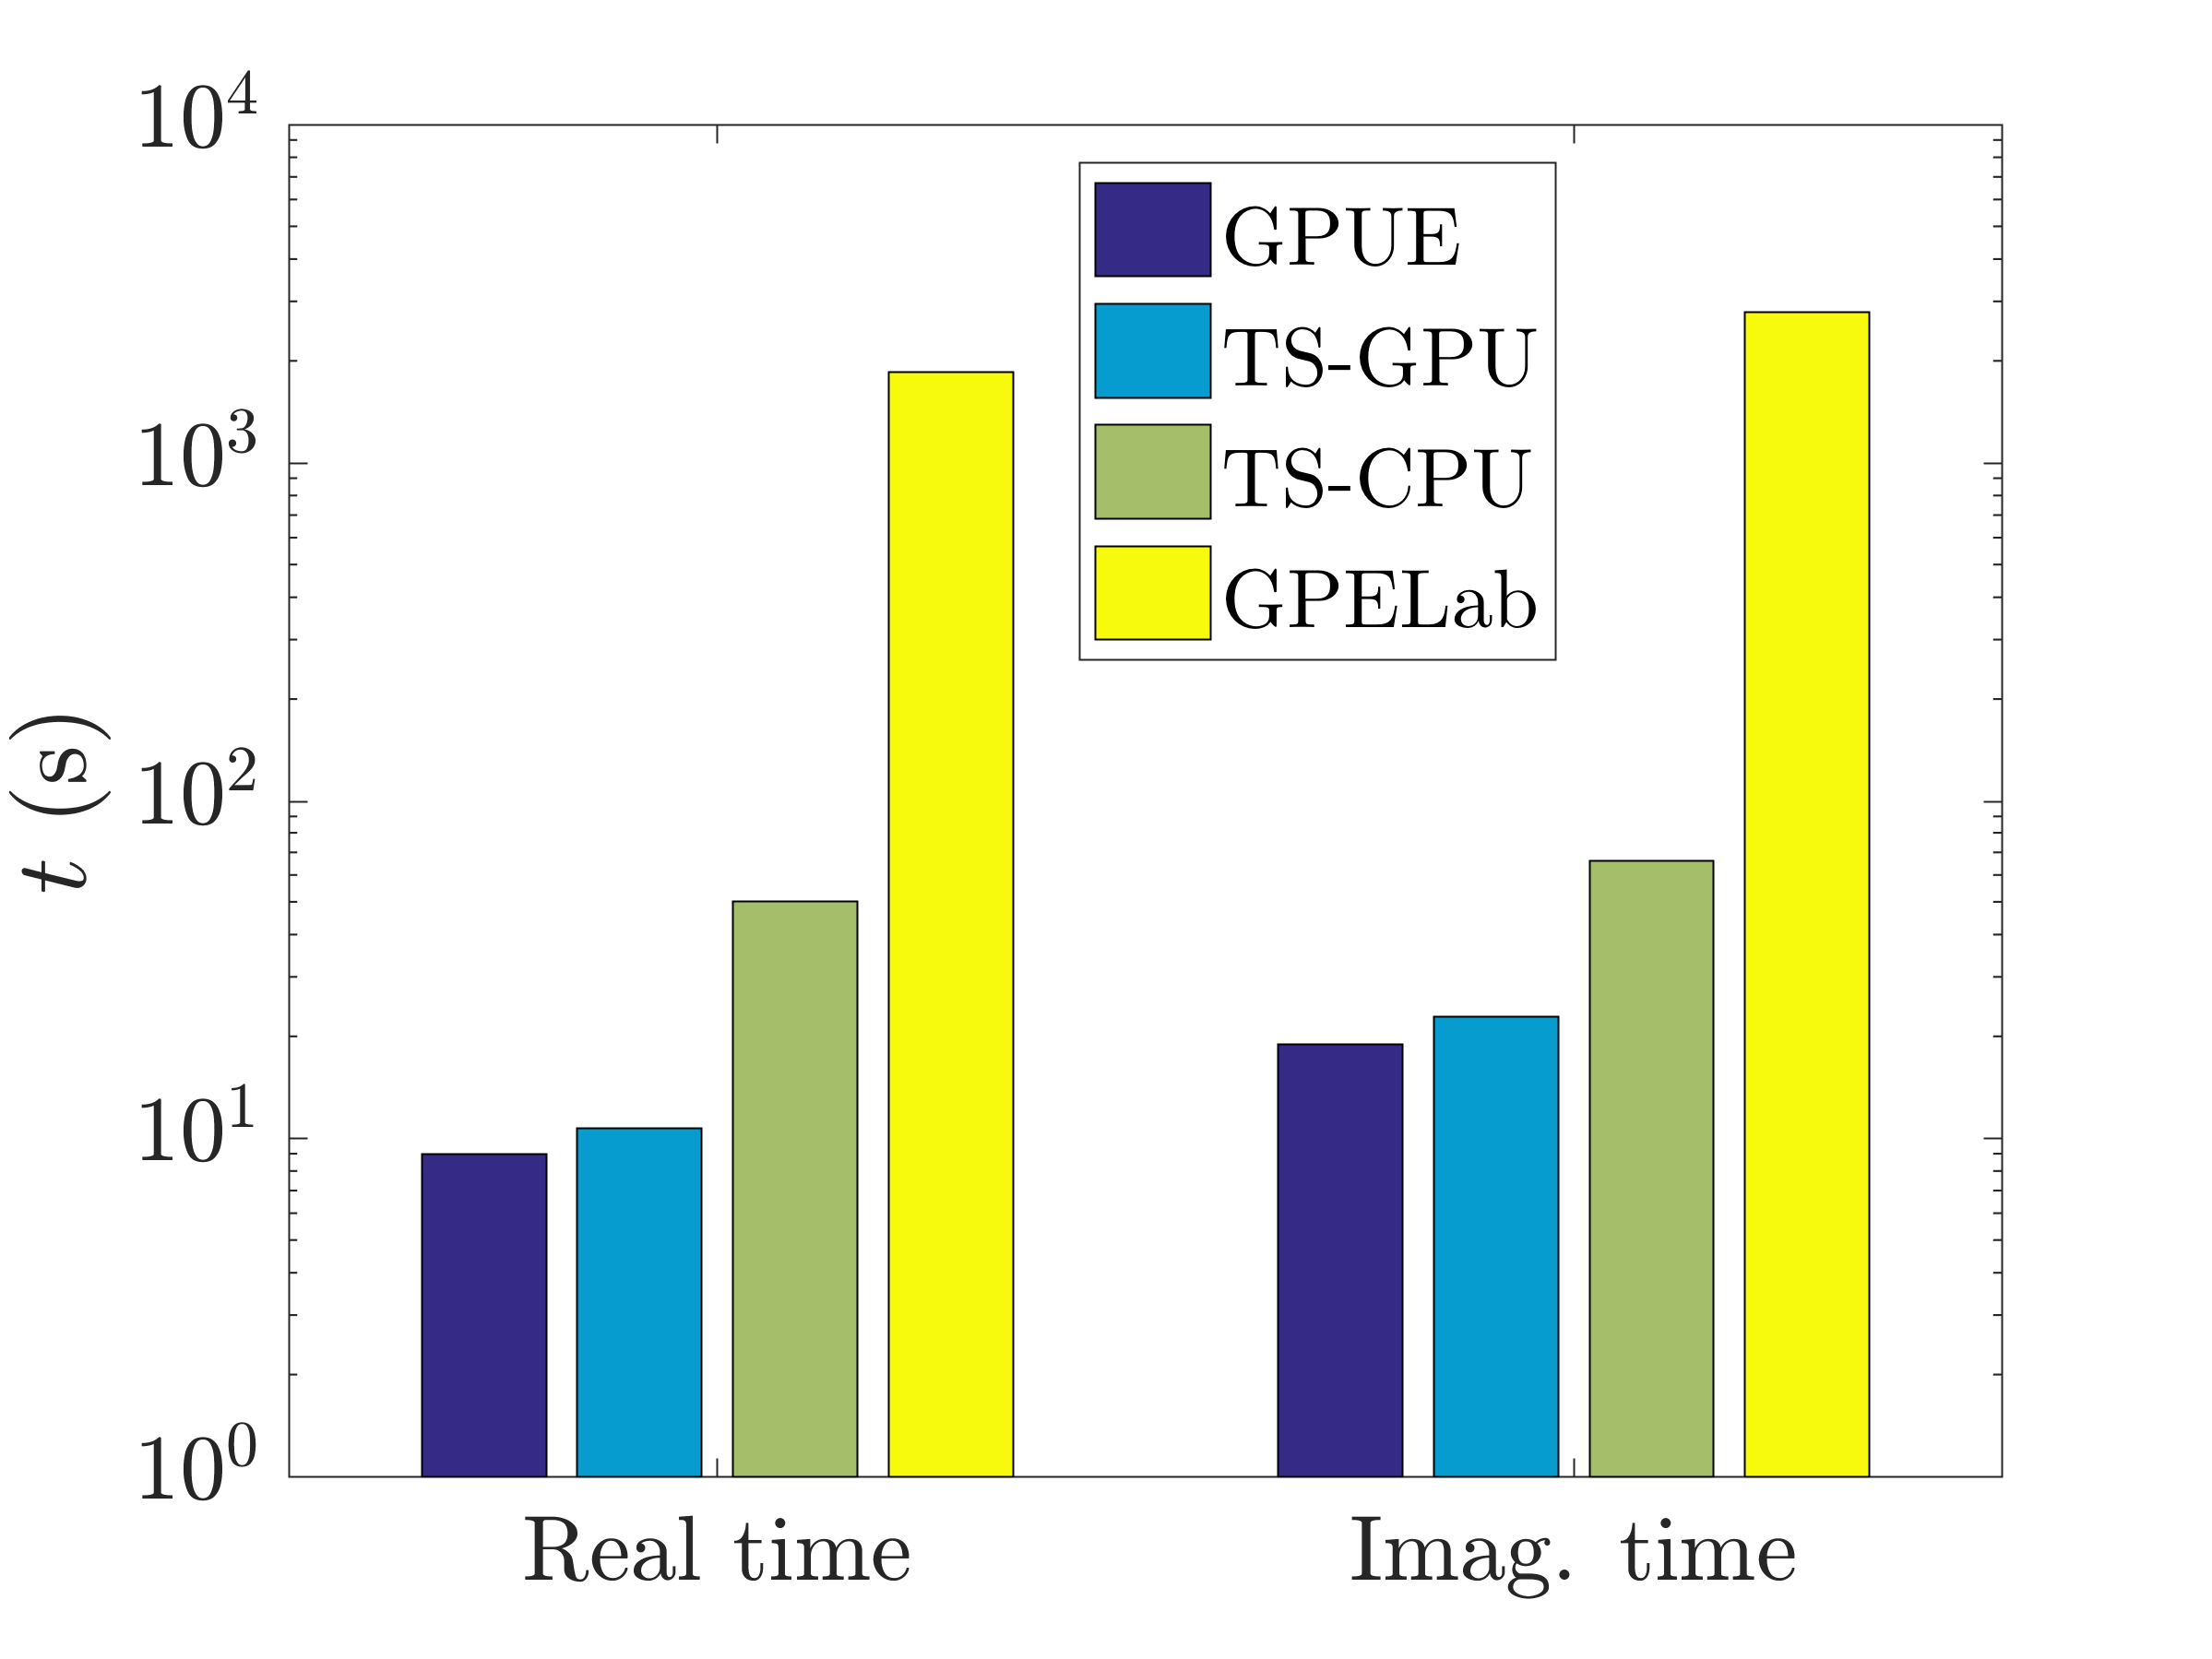
\includegraphics[width=0.7\textwidth,]{ch3_numerics/GPUEvsTS.png}
    \caption{Performance comparison of GPUE and other GPE simulation packages. Data adapted from [wittek url].}
    \label{fig:gpuevsts}
\end{figure}

A simplified sequence and state diagram combination is given in Fig.~\ref{gpue_seq} which describes the operating process for GPUE.

\begin{figure}[h]
    \centering
        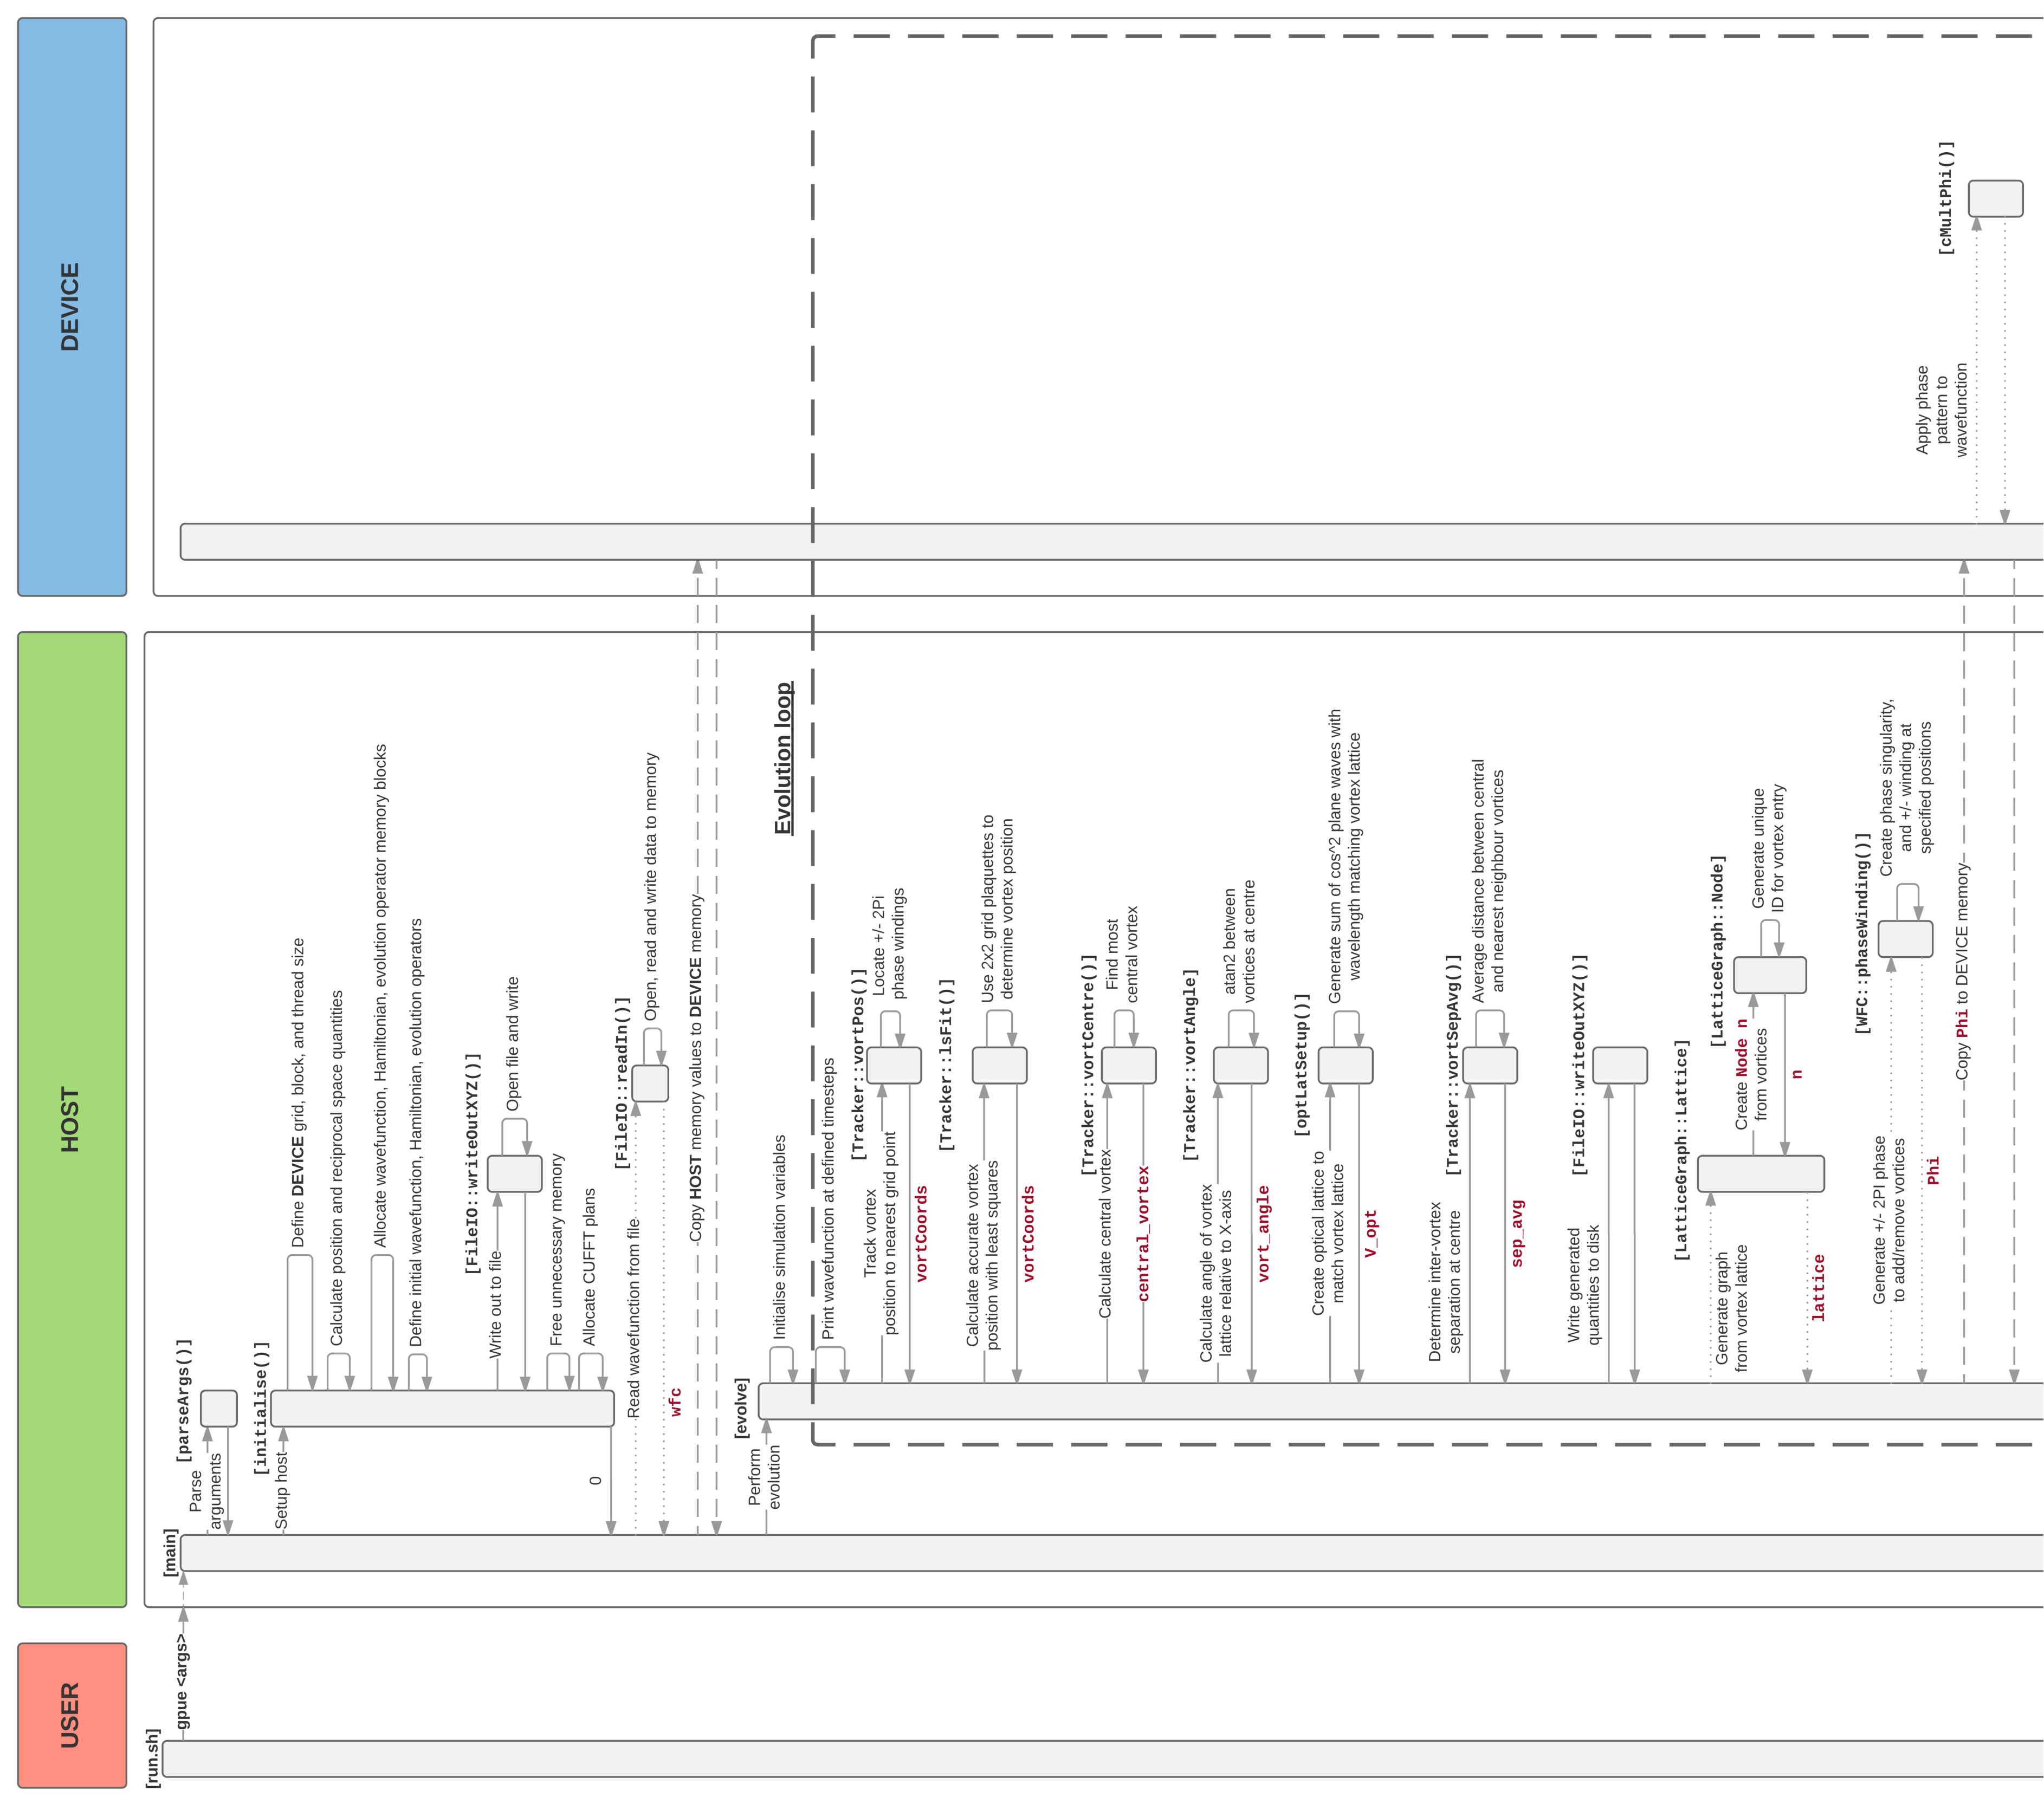
\includegraphics[height=\textwidth,angle=270]{ch3_numerics/GPUE_Seq1}
    \caption{Simplified combined sequence and state diagram for GPUE operation (1 of 2).}
    \label{fig:gpue_seq}
\end{figure}
\begin{figure}[h]
    \centering
        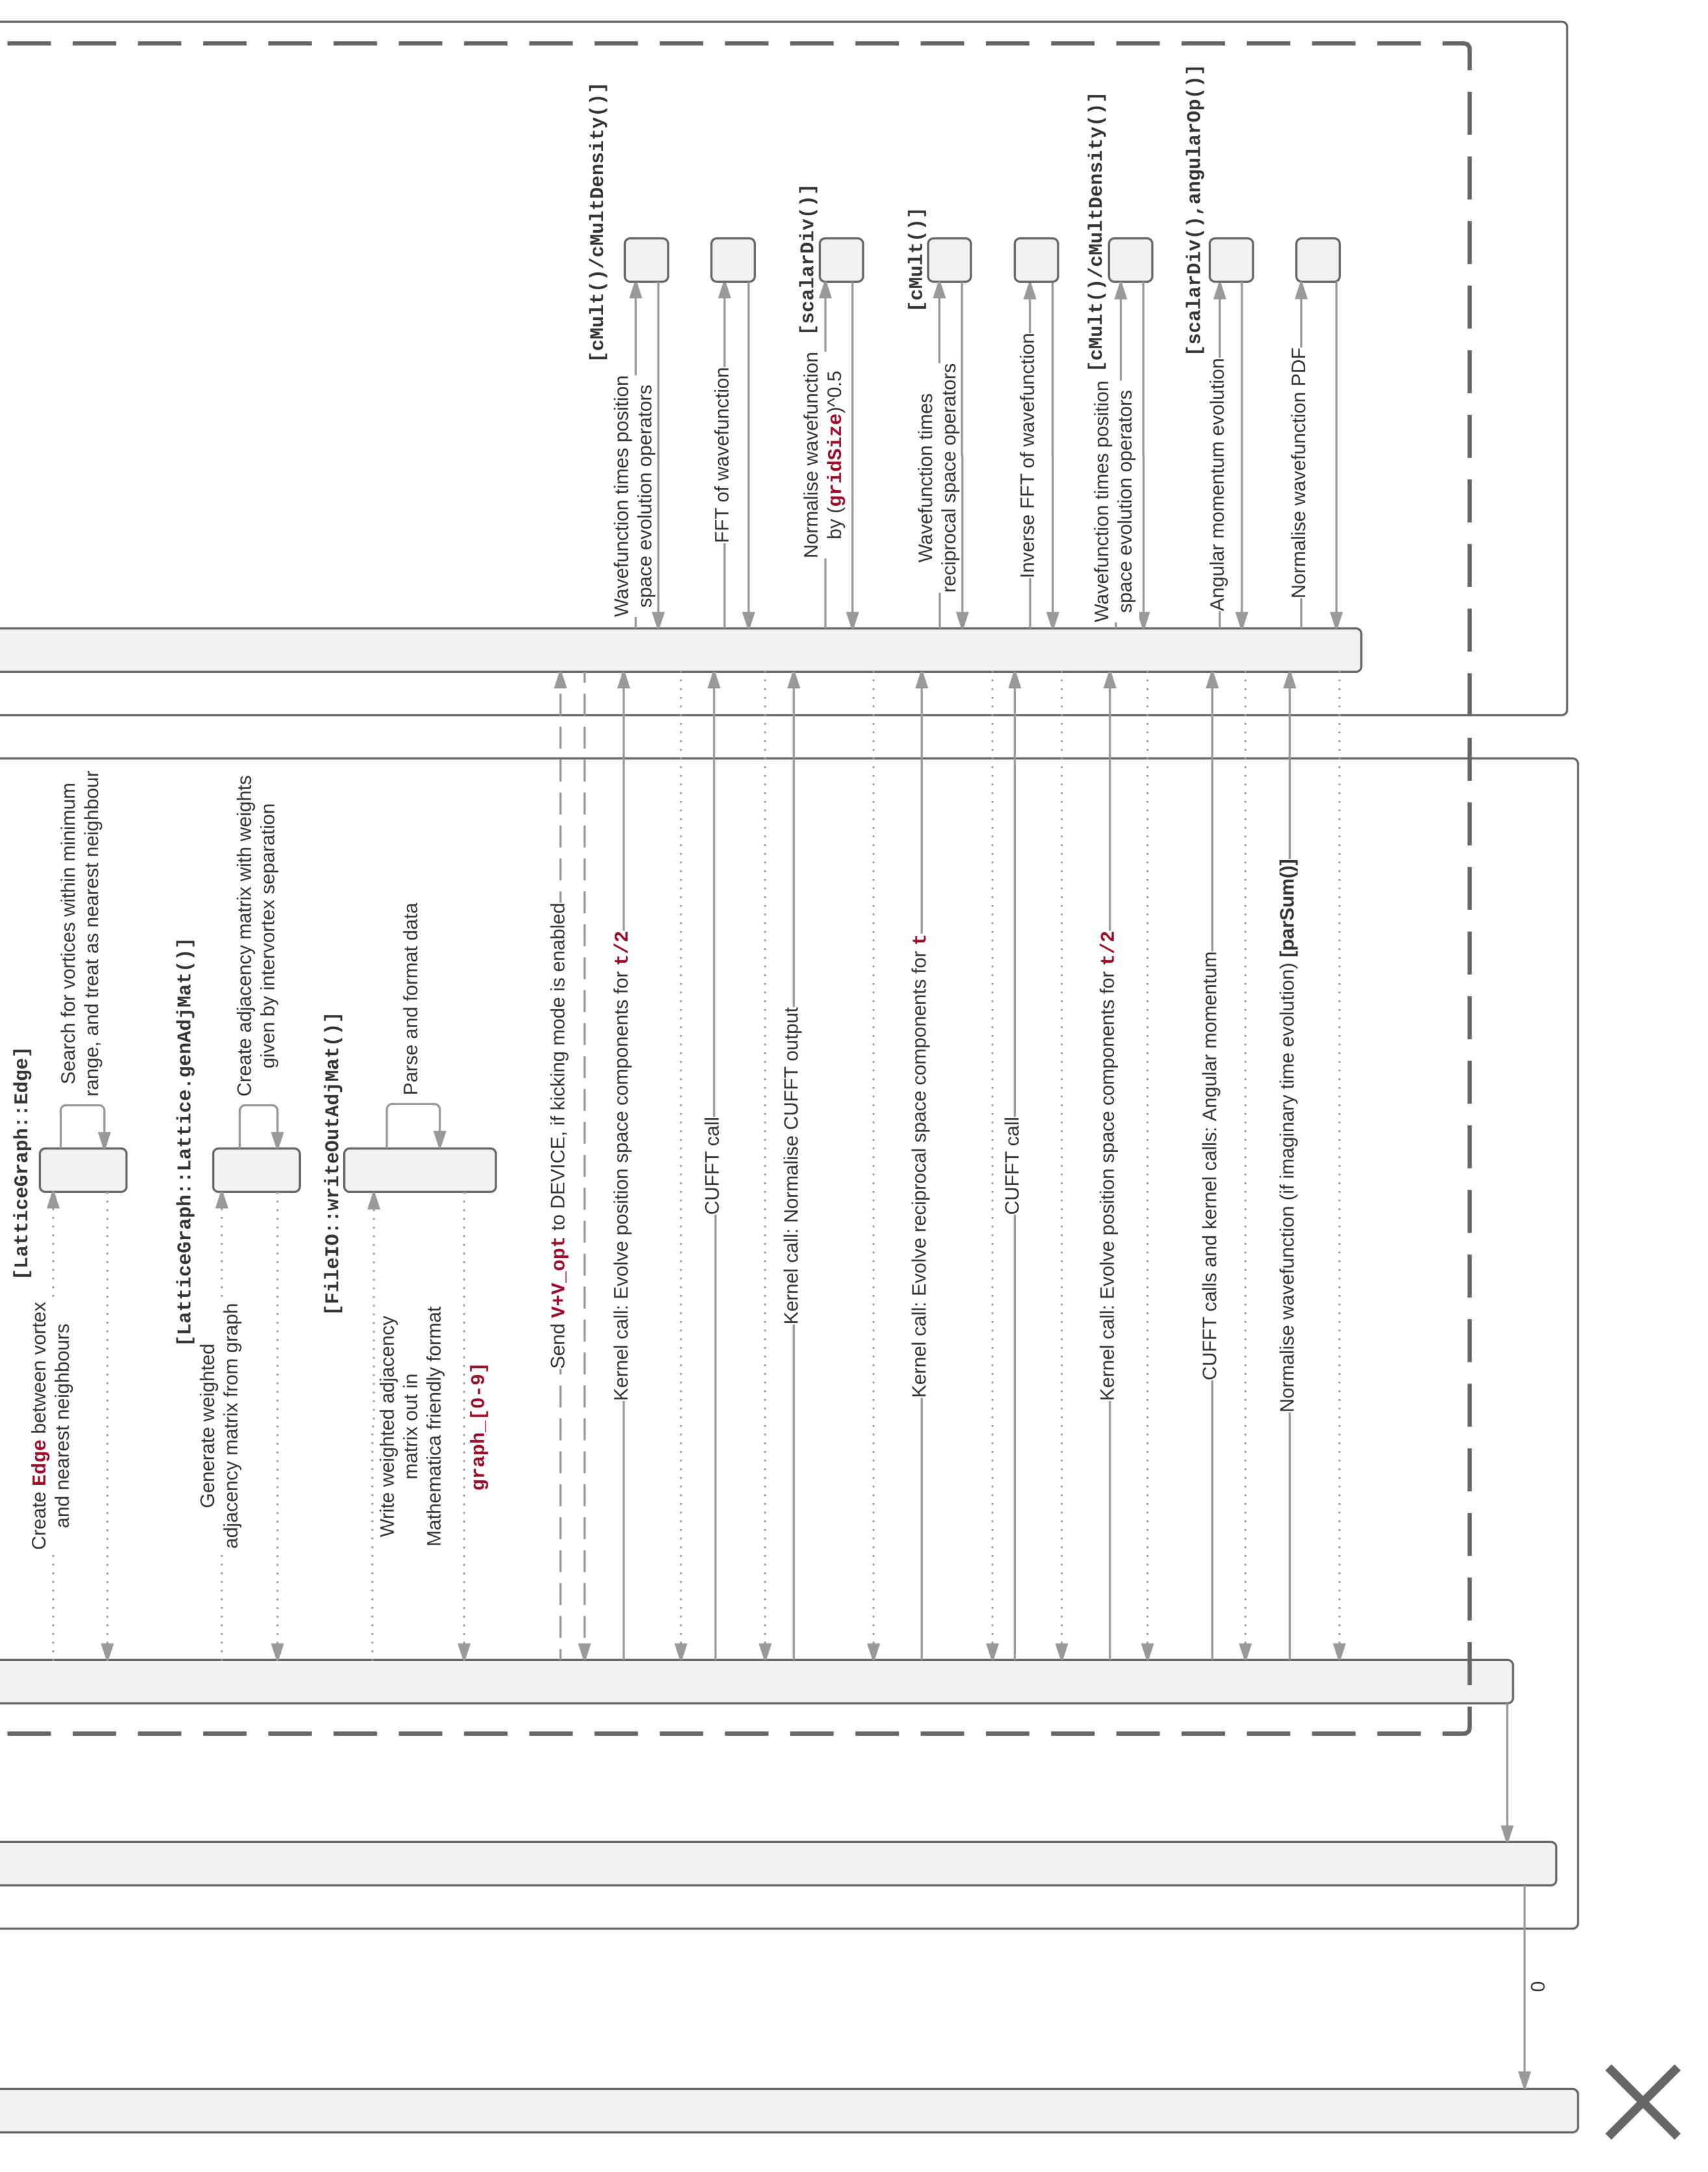
\includegraphics[height=\textwidth,angle=270]{ch3_numerics/GPUE_Seq2}
    \caption{Simplified combined sequence and state diagram for GPUE operation (2 of 2).}
    \label{fig:gpue_seq}
\end{figure}

\subsection{Angular momentum operators using Fourier split-operator (FSO) method}
In the presence of large values of angular momentum, the condensate wavefunction will accommodate many vortices. To ensure a well ordered lattice, it is insufficient to numerically solve the GPE at the required rotation rate. Assuming an initial Gaussian guess, the large number of vortices will enter the condensate from the edge and compete for lattice sites to form the expected Abrikosov pattern. Given the finite resolution and highly degenerate nature of the Abrikosov vortex lattice, it can take a significantly long time to reach and ordered state close to the transverse trapping frequency [Physical
Review Letters, 88(18):180403, (2002)]. Thus, to overcome this issue, I chose to follow the groundstate of the condensate with a ramp of the rotation rate. This is essentially adiabatic evolution during imaginary time, and for all required rotation rates of the condensate we get a vortex lattice ground-state. To allow for this we must examine the behaviour of the angular momentum operators within the FSO algorithm.

The FSO method described earlier works well in handling cases where the operators live in position or momentum space respectively. However, the angular momentum operators are essentially a combination of both spaces. Taking the angular momentum operator along the $z$-axis, $L_z = xp_y - yp_x$, to apply it to the wavefunction requires each basis elements be in the correct space, given the mixed dependencies. For applying this operator we must Fourier transform along a single dimension, multiply by the respective $\mathbf{k}$-space component, take the inverse, multiply by the respective $\mathbf{r}$-space component, and then perform this operation along the other dimensions, summing the results.

This approach accrues an error not encountered using methods solely in position or momentum space. The error can be determined by checking the commutativity of the respective components of the angular momentum operator as

 \begin{subequations}
 \begin{align}
 	\alpha_1 = [x p_y,-y p_x] &= [x p_y,-y] p_x  -  y[x p_y,p_x], \\
 				   &= -[-y,x p_y] p_x + y [p_x, x p_y], \\
 				   &= -\left( {\cancelto{0}{[-y,x]}} p_y + x [-y,p_y] \right) p_x + y \left( [p_x,x] p_y + x {\cancelto{0}{[p_x,p_y]}} \right), \\
 				   &= -x {\cancelto{i\hbar}{[-y, p_y]}} p_x + y {\cancelto{-i\hbar}{[p_x,x]}} p_y, \\
 				   &= -i\hbar \left(x p_x + y p_y \right).
 \end{align}
\end{subequations}

 The complex error term can be seen as, in the case of the implemented evolution, allowing the angular momentum operator to change from imaginary time to real-time, and vice-versa in each respective case. To overcome this, we simply swap the application order of the operator components, between even and odd steps during the evolution. Starting with the alternate order we obtain a value of $\alpha_2 = [-y p_x, x p_y] = i\hbar \left(x p_x + y p_y \right)$. Since we are applying these operators to the condensate we can overcome the error of one term by the application of the other, as
 \begin{equation}
 \exp{i \alpha_1}\exp{i \alpha_2} = 1.
 \end{equation}

 Although alternating will provide a cancellation of this error, it can be assumed that for large timesteps the error will have a non-insignificant contribution to the overall dynamics, as the wavefunction evolves from timestep to timestep. Thus, for this method to remain accurate we can perform the previous decomposition for a second-order accurate scheme.

 A sample wavefunction at a rotation of $\Omega = 0.995\omega_x$ is given by Fig.~\ref{fig:showingoff} showing the density and phase at a resolution of $2^{11}\times 2^{11}$. Although aliasing may be apparent in the phase, this is more likely due to the limited resolution of the computer monitor (printer).

 \begin{figure}
     \centering
     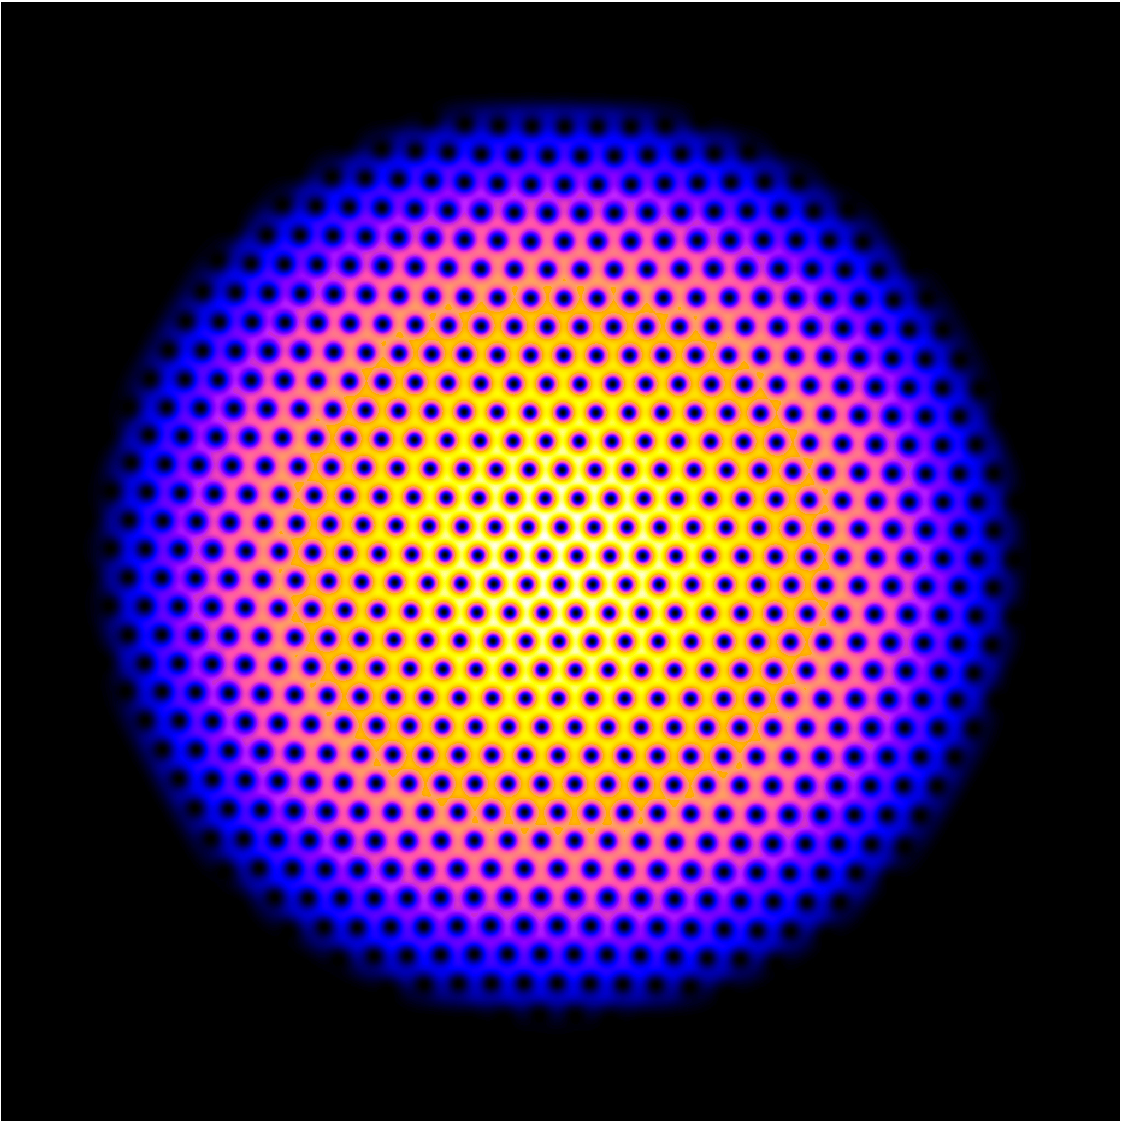
\includegraphics[width=0.45\textwidth,]{ch3_numerics/Rho_995}
     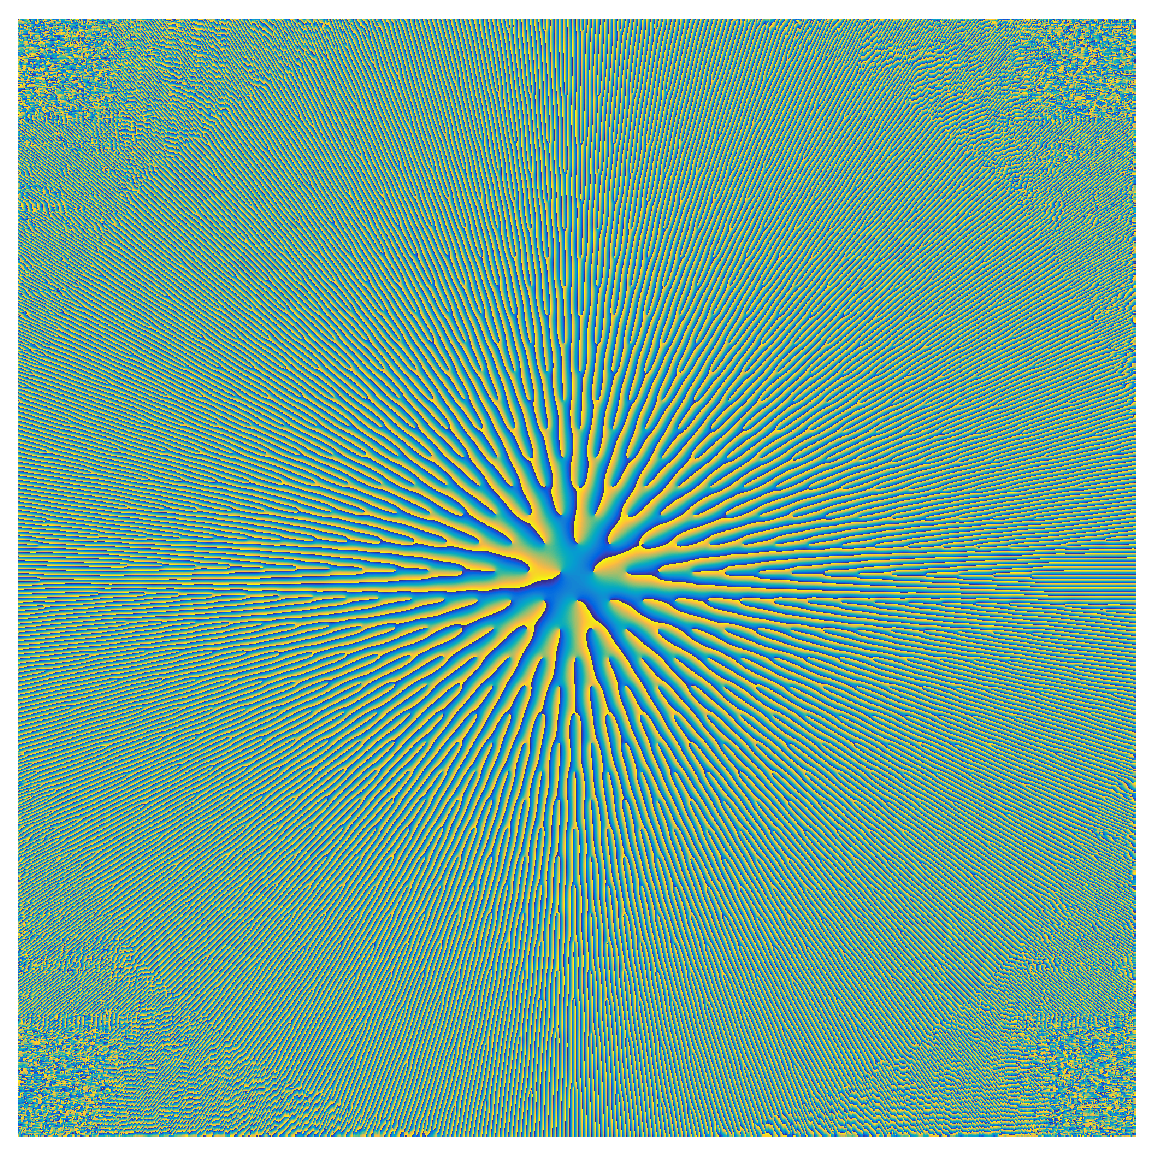
\includegraphics[width=0.45\textwidth,]{ch3_numerics/phi_995}
     \caption{Condensate density (L) and phase (R) at a rotation rate of $\Omega=0.995\omega_x$ for a $2^{11}\times 2^{11}$ grid showing approximately 600 vortices in the visible density regions.}
     \label{fig:showingoff}
 \end{figure}

 \subsection{Vortex tracking}
 To efficiently follow the vortex dynamics, some robust algorithm is needed to track their positions. One could track regions where the density drops to zero. However, this gives very little information on the topological excitation, and may mistake density dips such as phonons for the presence of such excitations. One of the most effective ways is to locate the $\pm 2\pi$ charge in the wavefunction phase, which is a signature of quantum vortices. We can assume that around a $2\times 2$ subgrid, the phase rotates from $-\pi$ to $+\pi$ in the presence of a vortex located on the subgrid. After an initial pass to determine the vortex locations closest the nearest grid element, a least-squares fit is performed to more accurately determine the vortex core position.

 Linear least squares is used generally for an overdetermined linear system $\mathbf{A}\mathbf{r} = \mathbf{b}$, where unique solutions are unlikely to exist. Thus, for a solution, we seek the best fit plane that minimises the error, of the form

 \begin{equation}
 S(\mathbf{r}) = \displaystyle\sum |b_i - \displaystyle\sum A_{ij} r_j |^2
 \end{equation}
 where $S$ is the objective function to be minimised, following $\mathbf{b} = \argmin S(\mathbf{r})$. The solution of this minimisation problem is given by
 \begin{subequations}
\begin{align}
    \mathbf{A} ^{T}\mathbf{A} \mathbf{r} &= \mathbf{A} ^{T}\mathbf{b}, \\
    \mathbf{r} &= (\mathbf{A}^{T}\mathbf{A})^{-1}\mathbf{A}^{T}\mathbf{b}.
\end{align}
\end{subequations}
For this the best-fit plane is sought of the form
$a_0 c + \displaystyle\sum\limits_{i}^{m} a_i r_i = f(\mathbf{r})$
which for a two-dimensional system, $\mathbf{r} = \{x,y\}$, is given by the matrix,
\begin{equation}
    \mathbf{A} = \left(
    \begin{array}{ccc}
        0 & 0 & 1 \\
        0 & 1 & 1 \\
        1 & 0 & 1 \\
        1 & 1 & 1
    \end{array}\right).
\end{equation}
The above matrix is composed of all possible planes that can fit over a square $2\times 2$ grid plaquette,
and
\begin{equation}
    \mathbf{b} = \left(
    \begin{array}{cccc}
        \Psi(x_0,y_0) & \Psi(x_0,y_1) & \Psi(x_1,y_0) & \Psi(x_1,y_1)
    \end{array} \right)^{T},
\end{equation}
are the wavefunction values around the sampled $2\times 2$ grid.
Upon evaluating the vector $\mathbf{r}$ above, one can obtain the best fit plane  solution as
\begin{equation}\left(
    \begin{array}{c}
        x \\
        y \\
        c
    \end{array}\right)
    = \left(
    \begin{array}{c}
        0.5( -\Psi(x_0,y_0) + \Psi(x_0,y_1) - \Psi(x_1,y_0) + \Psi(x_1,y_1) ) \\
        0.5( -\Psi(x_0,y_0) - \Psi(x_0,y_1) + \Psi(x_1,y_0) + \Psi(x_1,y_1) ) \\
        3\Psi(x_0,y_0) + \Psi(x_0,y_1) - \Psi(x_1,y_0) - \Psi(x_1,y_1) )
    \end{array}\right).
\end{equation}

The goal is to find where both the real and imaginary components cross through zero, and thus we seek a solution of the form $x + y = -c$. Rearranging the above equations as
\begin{equation}\left(
    \begin{array}{cc}
        \Re(x) & \Re(y) \\
        \Im(x) & \Im(y) \\
    \end{array}\right)
    \left(
    \begin{array}{c}
        \delta x \\
        \delta y
    \end{array}\right)
    =
    \left(
    \begin{array}{c}
        \Re(c)
        \Im(c)
    \end{array}\right).
\end{equation}
and again solving the linear system by inverting the left-hand matrix and multiplying across allows one to seek the corrections to the vortex position, $\delta \mathbf{r} = \{\delta x, \delta y \}$.

 With this, we can accurately determine the motion of the vortices with high precision. To track the vortices during the evolution, the creation of an initial list of vortices is performed, with each given a unique identifier. Assuming the vortex cores can travel a limited distance (some multiple of the grid resolution) between time steps, we can say at subsequent times which vortex has moved to the newly found positions.

 This is performed through representing vortices as a graph, each with an assigned unique identifier, associated location, phase winding and on/off flag. Edges are created between vortices that are separated by at most root-two the average of the inter-vortex spacings. A finite boundary is chosen to examine only vortices at the center, which can cause vortices to appear and disappear on the boundary. Thus, any vortex which appears without association to an initial vortex, or any vortex that leaves the boundary, is switched off and remains so for all analysis.
